\documentclass{article}
\usepackage{amsmath, amsfonts, amsthm, amssymb}  

\usepackage{secdot}
\usepackage{epsfig}
\usepackage[T1]{fontenc}
\usepackage{epstopdf}
\usepackage{url}
\usepackage{rotating}
\usepackage{graphicx}
\usepackage{caption}
\usepackage{subcaption}
\usepackage{multirow}
\usepackage{setspace}
\usepackage{array}
\usepackage{fancyhdr}
\usepackage{lastpage}
\usepackage[T1]{fontenc}

\usepackage{geometry}
\geometry{letterpaper, left=1in, right=1in, top=1in, bottom=1in}

\pagestyle{fancy}
\fancyhf{}
\rhead{\thepage/\pageref{LastPage}}
\lhead{OSU ECEN 4243 - Computer Architecture - Spring 2023}
\rfoot{\LaTeX}


% ----- Identifying Information -----------------------------------------------
\newcommand{\myassignment}{Lab 2: Debugging on the ELVIS III/DSDB boards}
\newcommand{\myinstructor}{Alex Underwood, Brett Mathis, Ross Thompson, and James E. Stine}
% -----------------------------------------------------------------------------

\begin{document}
\graphicspath{{.}{./latex_graphics/}}
\begin{center}
  {\huge \myassignment} \\
  \myinstructor \\
\end{center}

\section{Debugging on an FPGA}
Debugging a circuit as it runs on an FPGA is quite different from when
it is running in a simulation tool like ModelSim.  Unlike ModelSim,
where all the logic signals inside the circuit can be exposed and
easily added to a waveform viewer, FPGAs have no inherently easy way
of viewing all of their logic signals.  In fact, many logic signals
that exist in your Verilog may be optimized or implemented out of the
design in order for the circuit's logic to better fit with what an
FPGA can do.  The FPGA also runs off of a real clock signal in real
time, making slowly stepping through the circuit like ModelSim nearly
impossible.  Luckily, Xilinx FPGAs and Vivado include debugging tools
that make it possible to `see' what is going on with some caveats.

There are two major ways to debug on hardware in Vivado -
block-diagram-level debugging and Verilog-level debugging.  For this
project, you will use Verilog level debugging.

\section{Adding Debug Flags}
To debug a signal, you need to tell the synthesizer and implementer
that you want to preserve the signal.  This prevents it from being
optimized out later and also makes it easier to find later in the list
of signals.  To do this, you add the following flag statement to the
declaration line of a signal you wish to debug:
\begin{verbatim}
(* mark_debug = "true" *)
\end{verbatim}
You can only add this flag to the declaration line of a signal
(logic and input/output) such as in the following examples:
\begin{verbatim}
(* mark_debug = "true" *) input logic [31:0] Instr;
(* mark_debug = "true" *) logic              MemWrite_edge;
\end{verbatim}
	
Add this to every signal you wish to view while your circuit is
running on the FPGA and remember that if you want to see new signals,
you'll need to add flags to those as well and reprocess the changes
you've made.
	
\section{Setting up Debugging}
Once you've added the debug flags and saved/updated your changes to
the module, click `Run Synthesis' and wait for Block Generation and
Synthesis to complete.  We need to step in post-synthesis and modify a
few things before we continue running the toolchain, so don't jump to
Generate Bitstream yet or the debug flags will be ignored.  After
synthesis, open the synthesized design and select `Set up Debugging'.
This is where you will set up an Integrated Logic Analyzer that will
monitor your flagged signals and relay the information back to Vivado.
Select to start debugging only new nets and proceed.
\begin{figure} [h!]
  \centering
  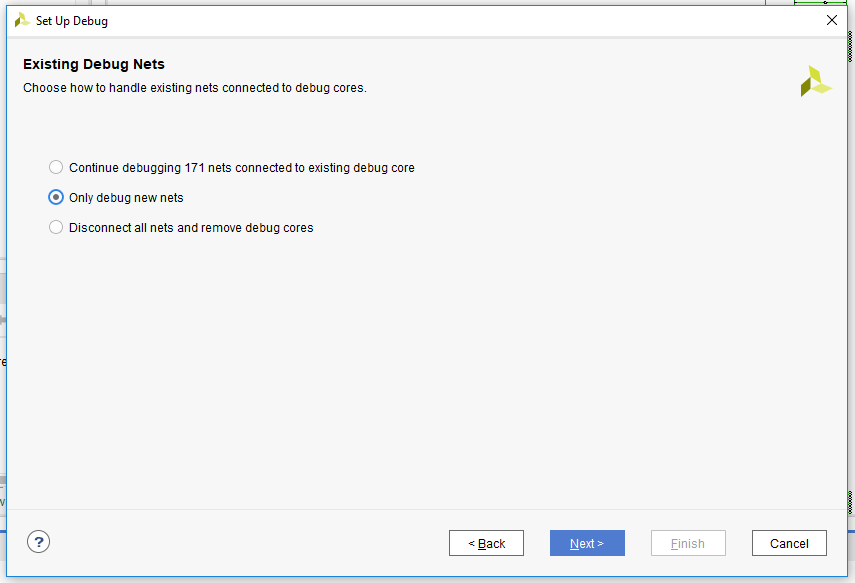
\includegraphics[scale=0.35]{figures/figure1.png}
\end{figure}	
	
If the signals you flagged don't show up on the list, use the `Find
Nets' search and change the filter to \verb|mark_debug| to add them to
the list.	
\begin{figure} [h!]
  \centering
  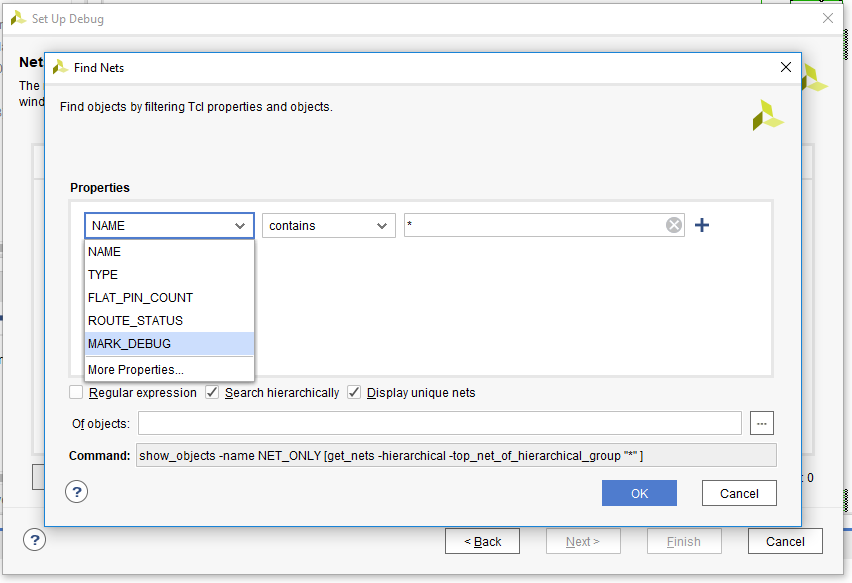
\includegraphics[scale=0.35]{figures/figure2.png}
\end{figure}	
	
Next, you can select how many samples of data you'd like to take with
each measurement.  Each sample represents a clock cycle, so the
default of 1024 will be fine for most of what we do in lab. However,
if you start using a significant number of signals to debug your
design, you may want to increase the sample depth. This is fine,
although this will require a slightly longer synthesis time.
\begin{figure} [h!]
  \centering
  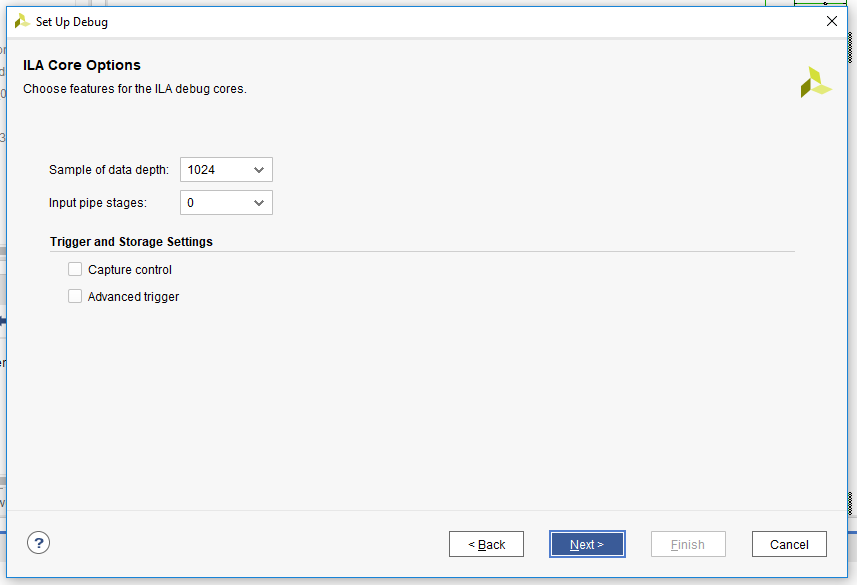
\includegraphics[scale=0.35]{figures/figure3.png}
\end{figure}	
	
Review the settings and then finish the debugger.  Now you can use
`Generate Bitstream' to finish running the remaining components of the
toolchain and get ready to upload to the FPGA. 	
	
\section{Using the Waveviewer}
Open the hardware manager and connect to the FPGA as usual.  Once your
FPGA has been programmed, the hardware manager will automatically
connect to the debugger on the FPGA and open the waveform viewer in
Vivado.  From here, the waveviewer is similar to ModelSim in the way
you can add signals (but only the ones you flagged earlier!) and
navigate the viewer.  But because this circuit is `running' all the
time on the FPGA, you will need to set up a trigger so the debugger
knows when to start taking data.
	
Use the trigger window to add one of the signals you flagged to be the
trigger, and then customize the behavior you want the trigger to
activate on.  This could be when the signal is 1, 0, rising or falling
edge, or any variety of bitwise and boolean operations.  You can also
combine multiple singals to form a trigger and select how you want
them to interact.
	
Once set up, click the start button to arm the trigger.  When armed,
the debugger will listen for the trigger you've set and collect data
upon activate.  That data is sent back to the waveviewer for you to
see on screen.  With the settings we've used, you'll get information
about what happen before and after the trigger was activated.  If the
trigger doesn't activate (no data appears and does not show up as
completed), double check your trigger settings.  If the condition you
set in the trigger is never met, no data will be taken.  It's possible
the trigger condition is invalid or there's an issue in the Verilog
that causes the trigger condition to never be reached.
	
With the trigger activated and the data dumped, you can use the
waveviewer to see the changes in logic values as the clock ticks and
decide if the signals are behaving as the should, going back to the
Verilog to adjust accordingly.
	
\section{Adding New Debug Signals}
If you want to go back and add more debug signals (or disable
debugging on other signals, don't forget to do that!), go back to the
Verilog and repeat adding new debug flags.  Synthesize the design and
use `Set up Debugging' with the option to `Only debug new nets'.  This
helps clean up old connections if you've removed debugging flags which
can cause errors later in the toolchain if not removed.  Continue on
as before after that to get back to hardware debugging.
	
\section{Helpful Tips}
\begin{itemize}
\item Think carefully about what would make a good trigger signal for
  what it is you're trying to debug.  Remember that the debugger will
  sava datapoints from before and after the trigger activates.
\item It is often helpful when debugging to draw out small parts of
  the circuit that you're focusing on and even make a few truth tables
  so you have down what you expect to happen and can easily compare
  with what's really happening.  Otherwise, it is easy to get lost in
  the waveviewer and miss important details.
\item Debugging increases how long it takes to run the toolchain, and
  the more signals you have flagged for debugging, the longer it
  takes!  Make sure you remove the debug flags from signals you are
  finished with so they don't slow down the toolchain later.
\item Nothing in the class labs will require you to debug signals at
  the block diagram level, so you do not need to add debug modules to
  the block diagram.
\item If you want to disable debugging entirely regardless of debug
  flags, you can select to `Remove all debug modules' in the `Set up
  Debugging' menu.  This will ignore the flags you have set up and
  continue running the rest of the toolchain as if they weren't there.  
\end{itemize}
	
\end{document}
